%%%%%%%%%%%%%%%%%%%%%%%%%%%%%%%%%%%%%%%%%%%%%%%%%%%%%%%%%%%%%%%%%%%%%%%%%%%%%%%%%%
\begin{frame}[fragile]\frametitle{}
\begin{center}
{\Large Introduction to Blockchain}
\end{center}
\end{frame}

%%%%%%%%%%%%%%%%%%%%%%%%%%%%%%%%%%%%%%%%%%%%%%%%%%%%%%%%%%%%%%%%%%%%%%%%%%%%%%%%%%
\begin{frame}[fragile]\frametitle{What on earth is Blockchain?}
\begin{itemize}
\item A blockchain is a digital concept to store data, in form of blocks, chained one after another.
\item Its public and immutable (non changeable)
\item Anything can be stored as data (to name some: property rights, identities, money balances, medical records), without being at risk of someone tampering with those records.
\end{itemize}


And there is an addition of one more word,  which is a must in every talk...and that is?


\end{frame}

%%%%%%%%%%%%%%%%%%%%%%%%%%%%%%%%%%%%%%%%%%%%%%%%%%%%%%%%%%%%%%%%%%%%%%%%%%%%%%%%%%
\begin{frame}[fragile]\frametitle{History}
\begin{itemize}
\item Initially came from Stuart Haber and W. Scott Stornetta (not the name though) 1991 paper ``How to Timestamp a digital document''.
\item Later, Satoshi Nakamoto in his Bitcoin paper, popularized the term 'Blockchain'
\end{itemize}
\end{frame}

%%%%%%%%%%%%%%%%%%%%%%%%%%%%%%%%%%%%%%%%%%%%%%%%%%%%%%%%%%%%%%%%%%%%%%%%%%%%%%%%%%
\begin{frame}[fragile]\frametitle{Definition}
{\emph A blockchain is a continuously growing list of records, called blocks, which are linked and secured using cryptography - Wikipedia}

\end{frame}


%%%%%%%%%%%%%%%%%%%%%%%%%%%%%%%%%%%%%%%%%%%%%%%%%%%%%%%%%%%%%%%%%%%%%%%%%%%%%%%%%%
\begin{frame}[fragile]\frametitle{}
\begin{center}
{\Large Concepts}
\end{center}
\end{frame}

%%%%%%%%%%%%%%%%%%%%%%%%%%%%%%%%%%%%%%%%%%%%%%%%%%%%%%%%%%%%%%%%%%%%%%%%%%%%%%%%%%
\begin{frame}[fragile]\frametitle{Block}
\begin{itemize}
\item Block is a set of data/records/transactions, previous block pointer or hash, value ie own hash
\item First block in the blockchain is called as Genesis block. It will remain forever. Does not have previous hash.
\item When blocks are linked, becomes a chain.
\end{itemize}

\end{frame}

%%%%%%%%%%%%%%%%%%%%%%%%%%%%%%%%%%%%%%%%%%%%%%%%%%%%%%%%%%%%%%%%%%%%%%%%%%%%%%%%%%
\begin{frame}[fragile]\frametitle{Hash}
\begin{itemize}
\item Fingerprints are unique to an individual (theoretically)
\item Similarly, Signatures (again, theoretically) to an individual.
\item Similarly, for data (string typically, but any type is fine), such unique signature is given by Hash function, popular one is SHA256
\item Hash is a number. Although you see some letters (A-F) in it, its because its a HEX number. You can do arithmetic with it.
\item Requirements for a good hash:
	\begin{itemize}
	\item One-way: From data to hash possible, but not the reverse way. Like from finger print you can not find how tall the person is, how s/he looks, etc.
	\item Deterministic: Even if you do Hashing multiple times, each time, same data gives same hash.
	\item Fast computation
	\item Avalanche effect: Even if a tiny change is made to data, the hash will be very different and not slightly different.
	\item Must withstand collision: no two data can have same hash.
	\end{itemize}
\item Smallest hash: `000 \ldots 000` (64 positions)
\item Highest hash: `FFF \ldots FFF` (64 positions)
\end{itemize}

\end{frame}

%%%%%%%%%%%%%%%%%%%%%%%%%%%%%%%%%%%%%%%%%%%%%%%%%%%%%%%%%%%%%%%%%%%%%%%%%%%%%%%%%%
\begin{frame}[fragile]\frametitle{Immutable Ledger}
\begin{itemize}
\item Example: Ownership of house is done by registering to Govt authority, name against the property in some central ledger.
\item Thats unsafe. Govt officials can tamper the records. Even digital/db records can be altered by admins.
\item Solution: Blockchain
\item Each transaction, buy/sell house, is stored in the Blockchain. It can not be tampered.
\end{itemize}

\end{frame}

%%%%%%%%%%%%%%%%%%%%%%%%%%%%%%%%%%%%%%%%%%%%%%%%%%%%%%%%%%%%%%%%%%%%%%%%%%%%%%%%%%
\begin{frame}[fragile]\frametitle{Distributed P2P Network}
\begin{itemize}
\item P2P: Peer to Peer
\item Every node in the network has the whole copy, so hard to manipulate all (at-least $> 51$\%).
\item Any computer/PC/Laptop can be part of the network.
\item All nodes are synced once a new transaction/block gets added.
\end{itemize}

\end{frame}

%%%%%%%%%%%%%%%%%%%%%%%%%%%%%%%%%%%%%%%%%%%%%%%%%%%%%%%%%%%%%%%%%%%%%%%%%%%%%%%%%%
\begin{frame}[fragile]\frametitle{Mining}
\begin{itemize}
\item Adding a new block (having a set of transactions) to existing blockchain.
\item Effort of adding the block needs to be rewarded. The effort is solving 'proof-of-work', solving a puzzle, getting n 0's in hash.
\item Apart from data/transactions and prev hash, there is a field called 'nonce' which when adjusted needs to come up a with block hash having certain number of leading zeros.
\item Whoever solves the puzzle first, gets to add the block to the blockchain and get some rewards in return.
\end{itemize}

\end{frame}

%%%%%%%%%%%%%%%%%%%%%%%%%%%%%%%%%%%%%%%%%%%%%%%%%%%%%%%%%%%%%%%%%%%%%%%%%%%%%%%%%%
\begin{frame}[fragile]\frametitle{Byzantine Fault Tolerance}
\begin{itemize}
\item Based on story of Byzantine castles,  where attacking generals have to come to consensus about the next action.
\item One of them is traitor. What protocol to be used?
\item Main general gives some order, then its decided to relay the same order to others, then majority decides the action.
\item If the commanding general himself is traitor, then he will have to issue at-least one opposite command to create confusion. In that case also the majority rule works fine.
\item COndition: not more that 30\% can be traitors.
\end{itemize}

\begin{center}
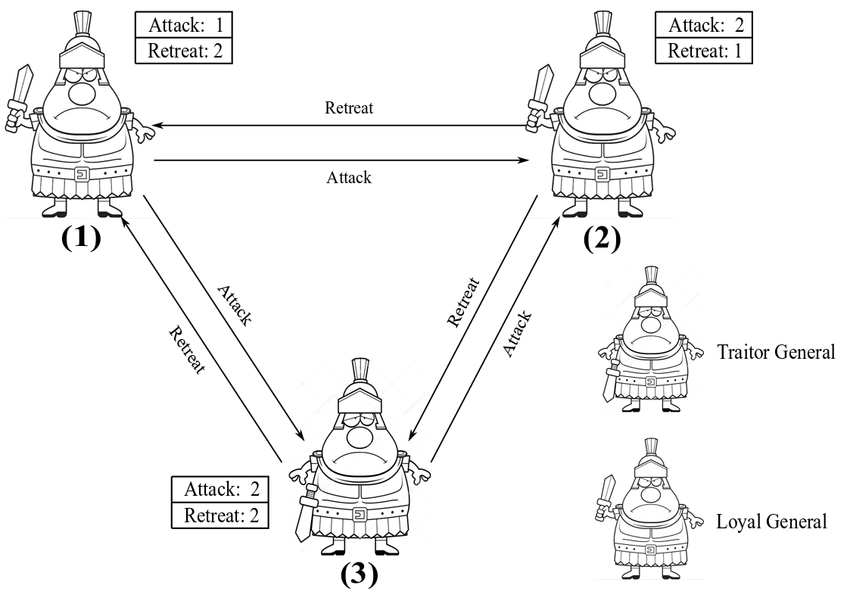
\includegraphics[width=0.6\linewidth,keepaspectratio]{blkchn_9}

{\tiny (Ref:``Byzantine problem with 3 generals. PBFT can only tolerate malicious'' - ResearchGate)}
\end{center}

\end{frame}

%%%%%%%%%%%%%%%%%%%%%%%%%%%%%%%%%%%%%%%%%%%%%%%%%%%%%%%%%%%%%%%%%%%%%%%%%%%%%%%%%%
\begin{frame}[fragile]\frametitle{Consensus Protocol: Defense Against Attackers}
\begin{itemize}
\item Attacker cannot put a block in the middle as s/he has t syn remaining nodes, which is impossible.
\item But can the malicious node be added at the end?
\item Every node does checks to verify the block, if fails, then the block gets rejected. No body gets reward.
\end{itemize}

\end{frame}

%%%%%%%%%%%%%%%%%%%%%%%%%%%%%%%%%%%%%%%%%%%%%%%%%%%%%%%%%%%%%%%%%%%%%%%%%%%%%%%%%%
\begin{frame}[fragile]\frametitle{Consensus Protocol: Competition Chains}
\begin{itemize}
\item Two chains which are far away, can mine a block at almost same time. Which one gets selected?
\item Many ideas: Proof-Of-Work (PoW) or Proof of Stake (PoS) or others
\item Only the one who wins the above challenge gets to mine the block.
\item They get some reward for the work done.
\item It may happen that some chains add blk1, some other chains add blk2, then which one is to be synced? SOlution is to wait for some time, see which chain is longest chain, that wins. It can be either with blk1 or blk2.
\end{itemize}

\end{frame}
